
\section{Approach}

\subsection{WW decay}

% -------------
% new frame
% -------------
\begin{frame}{Signal model: decay modes}

    The important parameters in our signal model are the W branching fractions,
    $$\vbw = \{\bwe, \bwm, \bwt, \bwh\},$$

    subject to the unitary constraint. Taking into account the \PGt decay modes, $\{\bte, \btm, \bth\}$, the \PW decay modes can be split further,

    $$\vbw^\prime = \{\bwe, \bwm, \bwt\bte, \bwt\btm, \bwt\bth, \bwh\}. $$

    All the possible terms for WW decays can be written in a matrix formed by the
    outer product of $\vbw^\prime$,

    \begin{equation*}
    \footnotesize
    \boldsymbol{B} =  \vbw^\prime\otimes \vbw^\prime =
    \begin{bmatrix}
        \bwe \bwe       & \bwe \bwm         & \bwe \bwt \bte        & \bwe \bwt \btm        & \bwe \bwt \bth        & \bwe \bwh         \\
        \bwm \bwe       & \bwm \bwm         & \bwm \bwt \bte        & \bwm \bwt \btm        & \bwm \bwt \bth        & \bwm \bwh         \\
        \bwt \bte \bwe  & \bwt \bte \bwm    & \bwt \bte \bwt \bte   & \bwt \bte \bwt \btm   & \bwt \bte \bwt \bth   & \bwt \bte \bwh    \\
        \bwt \btm \bwe  & \bwt \btm\bwm     & \bwt \btm \bwt \bte   & \bwt \btm \bwt \btm   & \bwt \btm \bwt \bth   & \bwt \btm \bwh    \\
        \bwt \bth \bwe  & \bwt \bth \bwm    & \bwt \bth \bwt \bte   & \bwt \bth \bwt \btm   & \bwt \bth \bwt \bth   & \bwt \bth \bwh    \\
        \bwh \bwe       & \bwh \bwm         & \bwh \bwt \bte        & \bwh \bwt \btm        & \bwh \bwt \bth        & \bwh  \bwh 
	\end{bmatrix} 
	\end{equation*}

    This results is a six-by-six symmetric matrix.

\end{frame}

% -------------
% new frame
% -------------
\begin{frame}{Signal model: templates}
    Correspondingly, there is a $6\times6$ symmetric matrix of the efficiencies\footnotemark for each decay mode to contribute to a specific final state,
    \begin{equation*}
    \footnotesize
    \boldsymbol{E} = \begin{bmatrix}
        \epsilon_{\Pe\Pe}       & \epsilon_{\Pe\PGm}        & \epsilon_{\Pe\PGte}       & \epsilon_{\Pe\PGtmu}          & \epsilon_{\Pe\PGth}       & \epsilon_{\Pe \mathrm{h}}   \\
        \epsilon_{\Pe\PGm}      & \epsilon_{\PGm\PGm}       & \epsilon_{\PGm\PGte}      & \epsilon_{\PGm\PGtmu}         & \epsilon_{\PGm\PGth}      & \epsilon_{\PGm \mathrm{h}}  \\
        \epsilon_{\Pe\PGte}     & \epsilon_{\PGm\PGte}      & \epsilon_{\PGte\PGte}     & \epsilon_{\PGte\PGtmu}        & \epsilon_{\PGte\PGth}     & \epsilon_{\PGte \mathrm{h}} \\
        \epsilon_{\Pe\PGtmu}    & \epsilon_{\PGm\PGtmu}     & \epsilon_{\PGte\PGtmu}    & \epsilon_{\PGtmu\PGtmu}       & \epsilon_{\PGtmu\PGth}    & \epsilon_{\PGtmu \mathrm{h}}\\
        \epsilon_{\Pe\PGth}     & \epsilon_{\PGm\PGth}      & \epsilon_{\PGte\PGth}     & \epsilon_{\PGtmu\PGth}        & \epsilon_{\PGth\PGth}     & \epsilon_{\PGth \mathrm{h}} \\
        \epsilon_{\Pe\mathrm{h}}& \epsilon_{\PGm\mathrm{h}} & \epsilon_{\PGte\mathrm{h}}& \epsilon_{\PGtmu\mathrm{h}}   & \epsilon_{\PGth\mathrm{h}}& \epsilon_\mathrm{hh}        \\
    \end{bmatrix},
    \end{equation*}

    %\vspace{-0.08in}
    \begin{tcolorbox}{}
        \smaller\smaller
        Putting this together, the predicted number of signal events in a final state is,

        \begin{equation}
            \nonumber
            n_{s} = \sigma_{s} \mathcal{L} \mathbf{E}_{ij} \mathbf{B}_{ij}. 
        \end{equation}

        The efficiencies are determined from simulated events,

        \begin{equation}
            \nonumber
            \epsilon = \frac{\sum_{\sf i\in acc.}w_{i}}{N_{total}}.
        \end{equation}

    \end{tcolorbox}

    \footnotetext[5]{\alert{\tiny N.B. W+jets accounted for just using the vector $\beta$ and the
    corresponding vector of efficiencies.}}

\end{frame}


% -------------
% new frame
% -------------
\begin{frame}{}%Frame Title}
    \begin{center}
        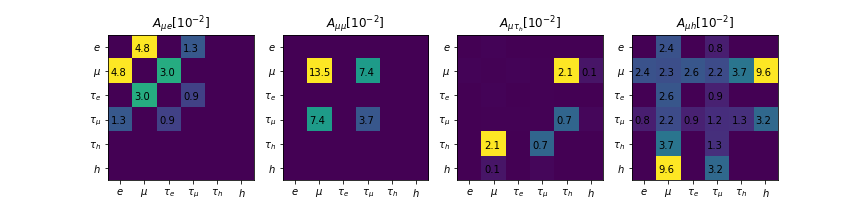
\includegraphics[width=0.9\textwidth,trim=3cm 0 3cm 0, clip]{chapters/Analysis/sectionStatisticalAnalysis/figures/acc_mu1b.png}
        % 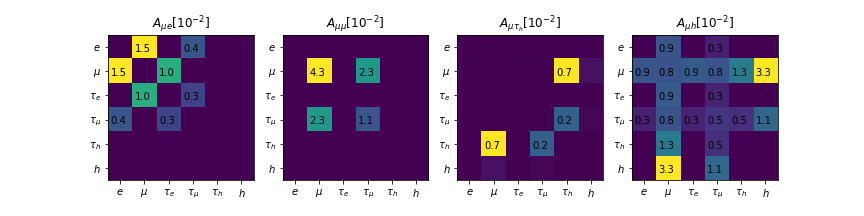
\includegraphics[width=0.7\textwidth]{chapters/Analysis/sectionStatisticalAnalysis/figures/acc_mu2b.png}
        % 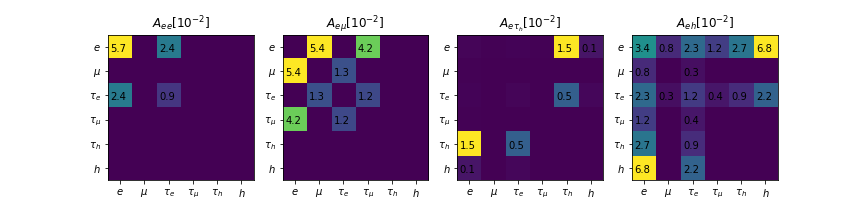
\includegraphics[width=0.7\textwidth]{chapters/Analysis/sectionStatisticalAnalysis/figures/acc_e1b.png}
        % 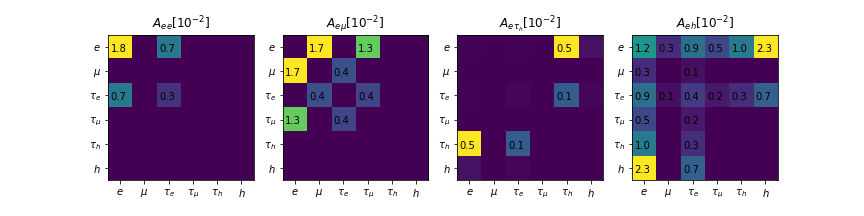
\includegraphics[width=0.7\textwidth]{chapters/Analysis/sectionStatisticalAnalysis/figures/acc_e2b.png}
    \end{center}
\end{frame}




\subsection{counting}

% -------------
% new frame
% -------------
\begin{frame}{}
    \begin{figure}
        \centering
        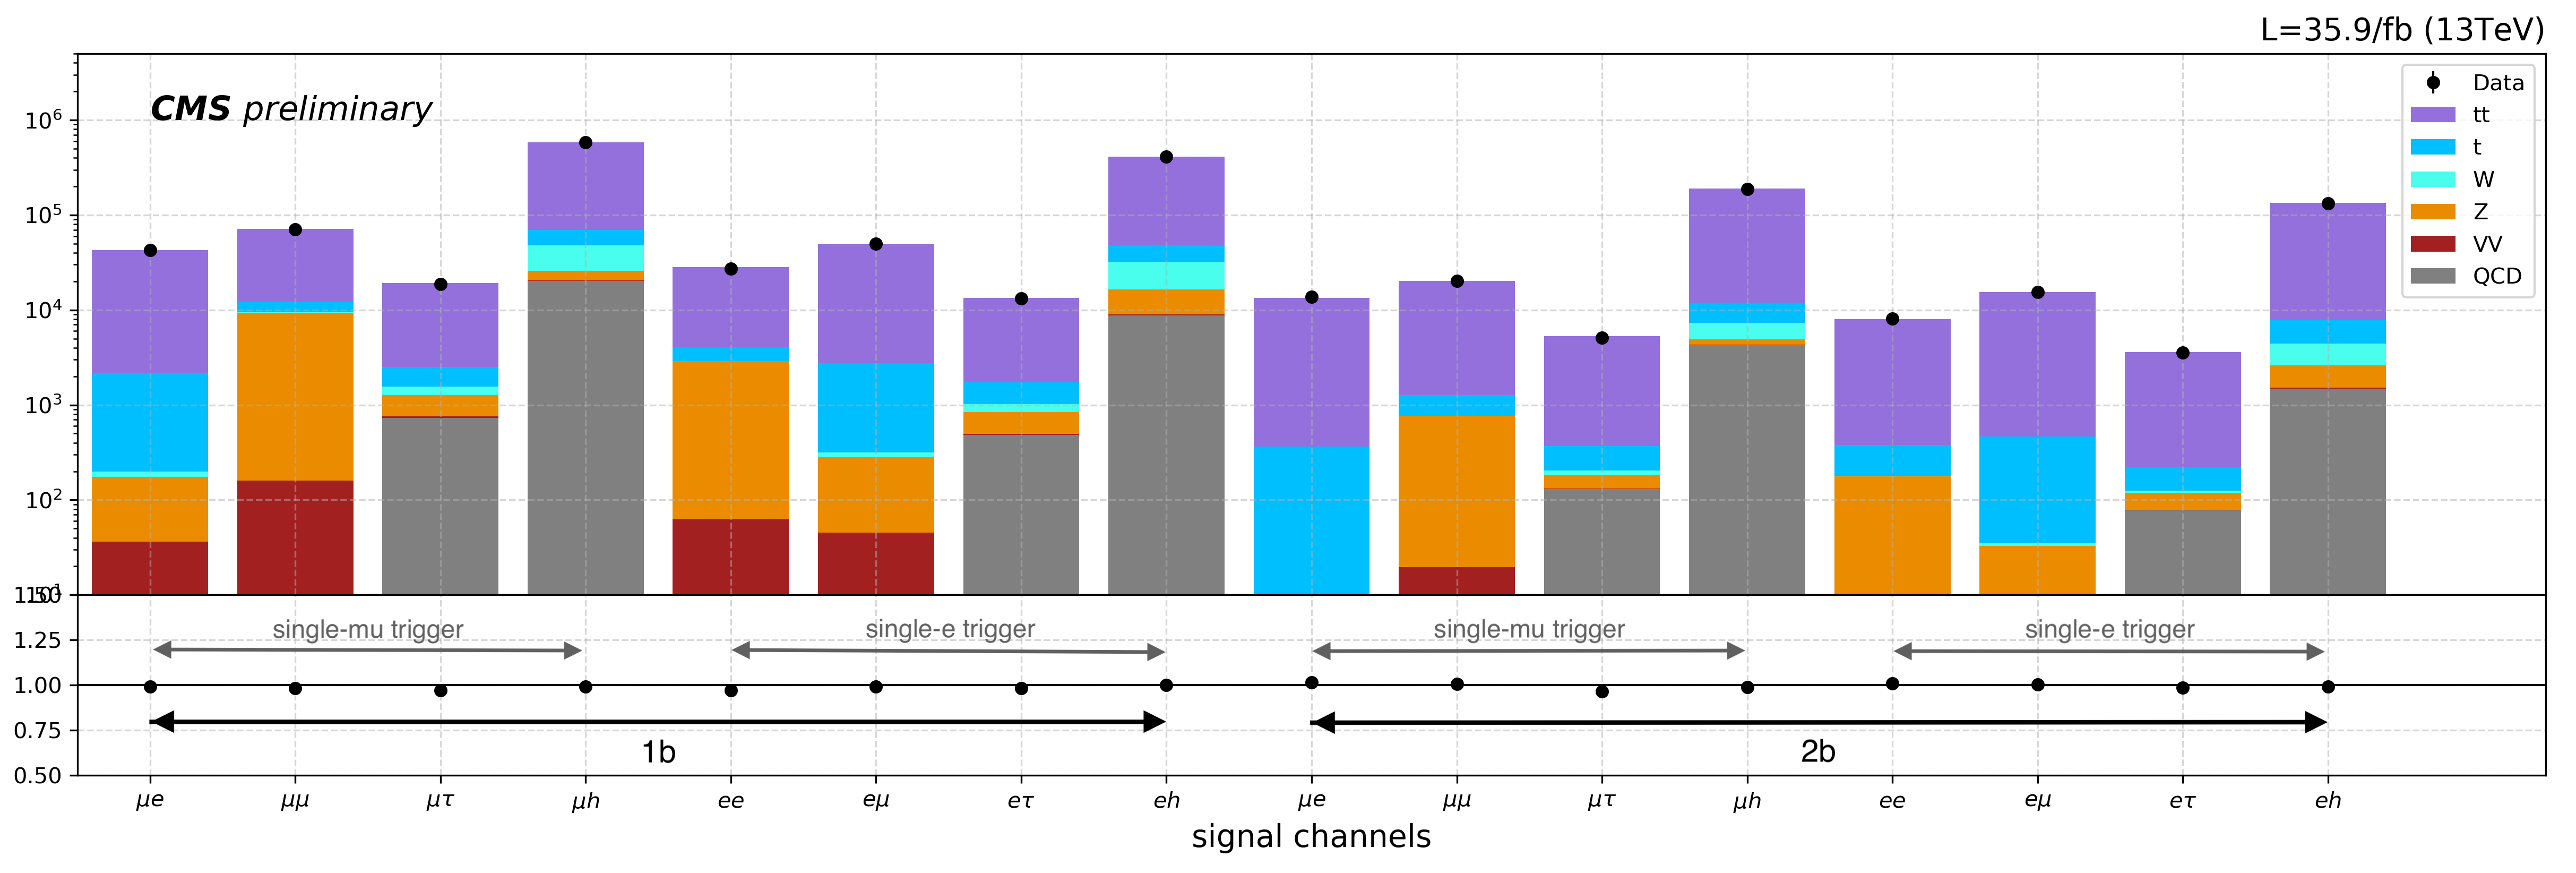
\includegraphics[width=0.9\textwidth]{chapters/Analysis/sectionStatisticalAnalysis/figures/counting.png}
    \end{figure}

    \smaller
    For each of the trigger and $n_b$ regions, construct ratios $\{X_{e},X_{\mu},X_{\tau}\}$ from
    data with background subtracted $n = N_{\rm data} - \sum N_{\rm bg}$,
    % Please add the following required packages to your document preamble:

    \begin{table}[]
        \centering
        \setlength{\tabcolsep}{2 em}
        \renewcommand{\arraystretch}{2}
        \resizebox{0.8\textwidth}{!}{
        \begin{tabular}{c|c|c|c|c}
        \rowcolor{NUpurple} 
                                & \multicolumn{2}{c|}{\textcolor{white}{Single-$\mu$ Trigger}}  & \multicolumn{2}{c}{\textcolor{white}{Single-$e$ Trigger}}    \\
        \rowcolor{NUpurple10} 
                                & $n_b = 1$                    & $n_b \geq 2$                   & $n_b = 1$                          & $n_b \geq 2$     \\ \hline 
        channels                & \multicolumn{2}{c|}{$\mu e$, $\mu \mu$, $\mu \tau_h$, $\mu h$} & \multicolumn{2}{c}{$e e$, $e \mu$, $e \tau_h$, $e h$}\\ \hline 
        \multirow{3}{*}{ratios, $t\in \{ \mu, e\}$} 
                                & \multicolumn{4}{c}{$\frac{n^{\ctre}  }{n^{\ctre} + n^{\ctrm} + n^{t\PGt} + n^{\ctrh}} = X_\Pe   = \frac{ \Eij^{\ctre}\Bij }{  \Eij^{\ctre}\Bij+ \Eij^{\ctrm}\Bij+ \Eij^{t\PGt}\Bij+ \Eij^{\ctrh}\Bij}$ } \\
                                & \multicolumn{4}{c}{$\frac{n^{\ctrm}  }{n^{\ctre} + n^{\ctrm} + n^{t\PGt} + n^{\ctrh}} = X_\PGm  = \frac{ \Eij^{\ctrm}\Bij }{  \Eij^{\ctre}\Bij+ \Eij^{\ctrm}\Bij+ \Eij^{t\PGt}\Bij+ \Eij^{\ctrh}\Bij}$ } \\
                                & \multicolumn{4}{c}{$\frac{n^{t\PGt}  }{n^{\ctre} + n^{\ctrm} + n^{t\PGt} + n^{\ctrh}} = X_\PGt  = \frac{ \Eij^{t\PGt}\Bij }{  \Eij^{\ctre}\Bij+ \Eij^{\ctrm}\Bij+ \Eij^{t\PGt}\Bij+ \Eij^{\ctrh}\Bij}$} 
        \end{tabular}
        }
    \end{table}
    
   
\end{frame}



% -------------
% new frame
% -------------
\begin{frame}{}%Frame Title}

    One gets a system of three quadratic equations with three unknowns $\{\bwe,\bwm,\bwt\}$,

    \begin{equation*}
    \tiny
	\begin{split}
        \textcolor{RedOrange}{F_\Pe(\bwe,\bwm,\bwt)} = c_{\Pe1} \bwe^2 + c_{\Pe2} \bwm^2 + c_{\Pe3} \bwt^2 + c_{\Pe4} \bwe\bwm + c_{\Pe5} \bwe\bwt + c_{\Pe6} \bwm\bwt + c_{\Pe7} \bwe + c_{\Pe8} \bwm + c_{\Pe9} \bwt + c_{\Pe0} &= 0 ,\\
        \textcolor{Blue}{F_\PGm(\bwe,\bwm,\bwt)} = c_{\PGm 1} \bwe^2 + c_{\PGm 2} \bwm^2 + c_{\PGm 3} \bwt^2 + c_{\PGm 4} \bwe\bwm + c_{\PGm 5} \bwe\bwt + c_{\PGm 6} \bwm\bwt + c_{\PGm 7} \bwe + c_{\PGm 8} \bwm + c_{\PGm 9} \bwt + c_{\PGm 0} &= 0, \\
        \textcolor{OliveGreen}{F_\PGt(\bwe,\bwm,\bwt)} = c_{_\PGt1} \bwe^2 + c_{\PGt2} \bwm^2 + c_{\PGt3} \bwt^2 + c_{\PGt4} \bwe\bwm + c_{\PGt5} \bwe\bwt + c_{\PGt6} \bwm\bwt + c_{\PGt7} \bwe + c_{\PGt8} \bwm + c_{\PGt9} \bwt + c_{\PGt0} &= 0 , \\
    \end{split}
    \end{equation*}
    
    where the coefficients $\{c_{ek},c_{\mu k},c_{\tau k} \}$ with $k\in\{ 0,1,2,\dots 9\}$ are fully determined by efficiencies $E$ and data ratios $\{X_e,X_\mu,X_\tau\}$.


	\begin{columns}[c] % align columns

	\column{.45\textwidth}
		\begin{figure}
			\centering
			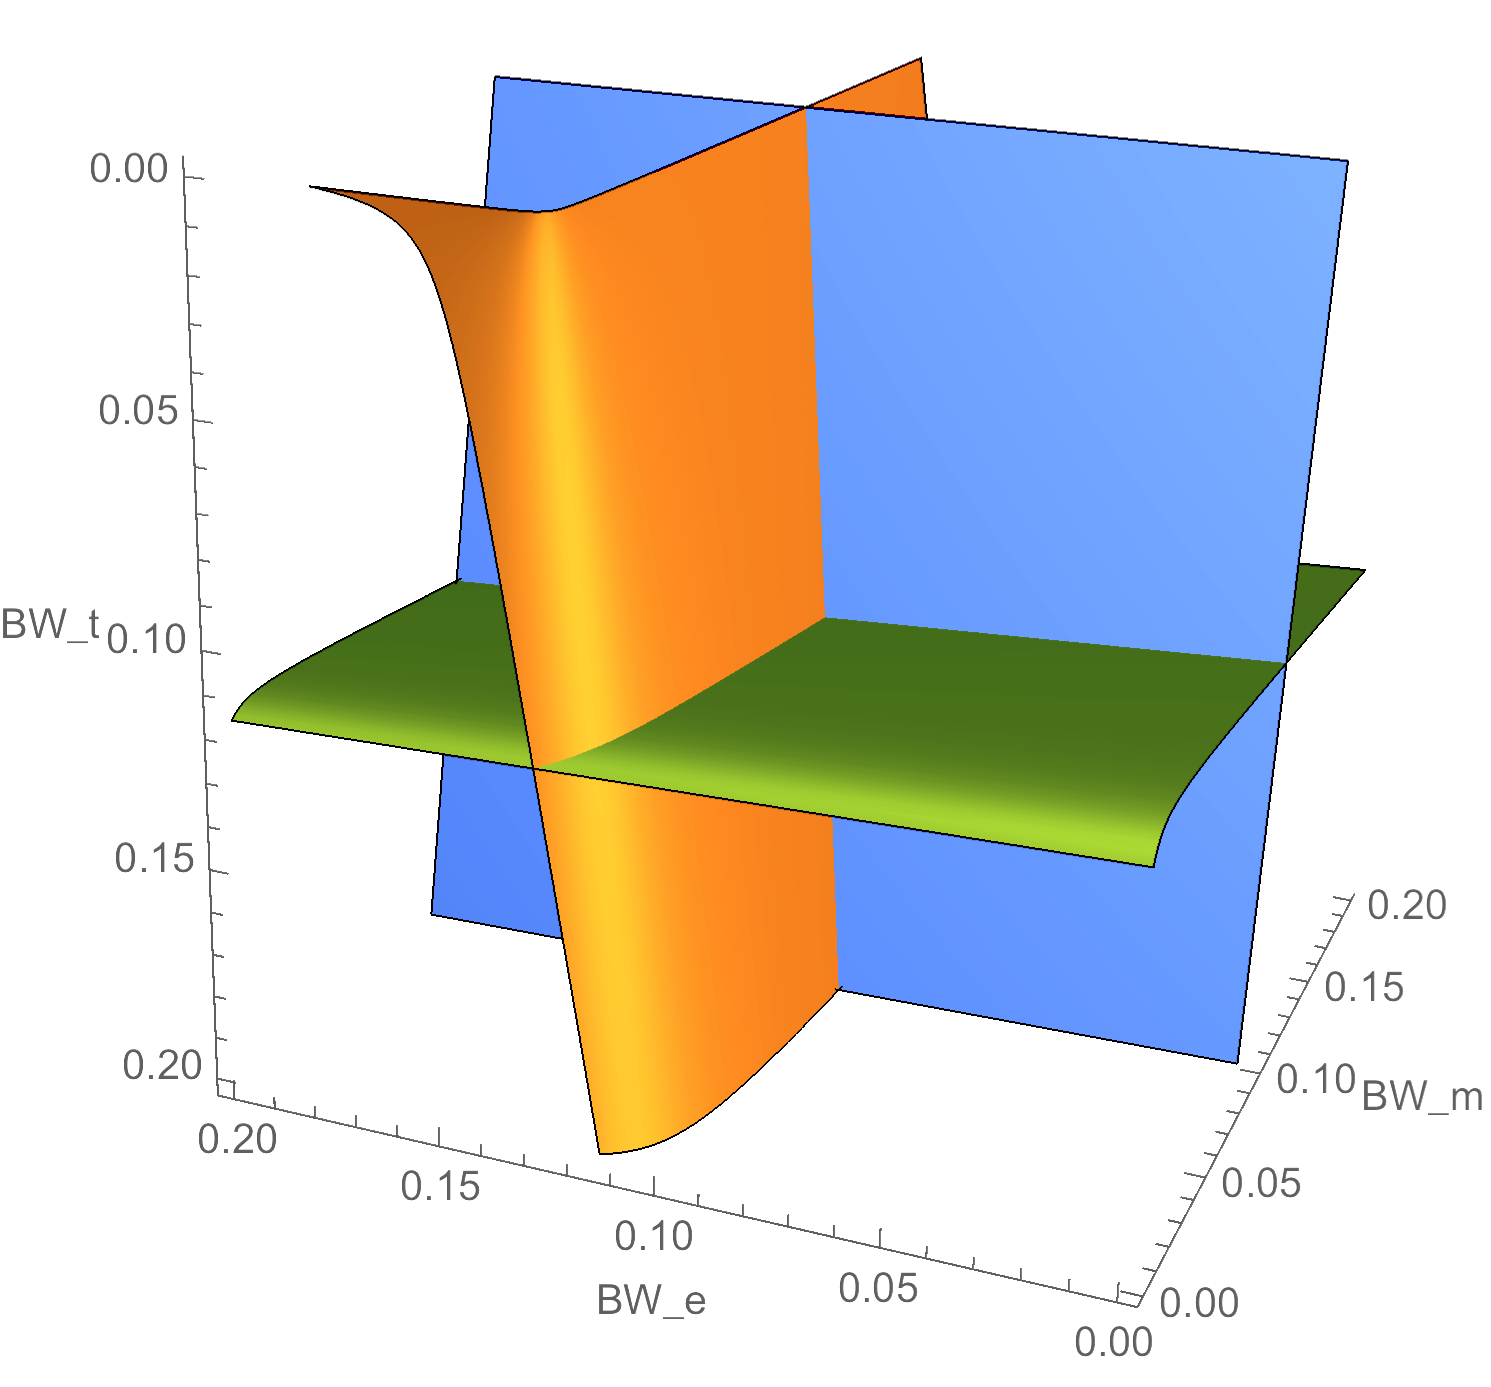
\includegraphics[width=0.9\textwidth]{chapters/Analysis/sectionStatisticalAnalysis/figures/visual.png}
		\end{figure}


	\column{.55\textwidth}
    \begin{itemize}
        \smaller
        \item In the $\{\beta_{e},\beta_{\mu},\beta_{\tau}\}$ space, three quadratic equations are three hyperbolic planes, intersection of which is the solution.
        
		\begin{equation*} 
            \small
            \begin{bmatrix} \bwe \\ \bwm \\ \bwt \end{bmatrix} = \text{Sol} 
                \begin{bmatrix}
                \textcolor{RedOrange}{F_\Pe (\bwe,\bwm,\bwt) = 0} \\
                \textcolor{Blue}{F_\PGm  (\bwe,\bwm,\bwt) = 0} \\
                \textcolor{OliveGreen}{F_\PGt (\bwe,\bwm,\bwt) = 0}
                \end{bmatrix}
		\end{equation*}

        \item The results from different data catagories are analytically combined considering the uncorrelated statistical error and correlated systematic errors.  
        \end{itemize}

	\end{columns}

\end{frame}

\begin{frame}{combine}
\smaller
    The systematic uncertainties are estimated by the changes of $\{\beta_{e},\beta_{\mu},\beta_{\tau}\}$ when variating up/down the systematical parameters by their $\pm 1\sigma$ uncertainties.
    The four solutions from the four the trigger-$n_b$ regions, $\mu 1b$, $\mu 2b$, $e1b$, $e2b$
    \begin{equation*}
        \tiny
        \beta_0 = \bigg [
        \beta_e^{\mu1b}, \beta_\mu^{\mu1b}, \beta_\tau^{\mu1b}, \quad 
        \beta_e^{\mu2b}, \beta_\mu^{\mu2b}, \beta_\tau^{\mu2b}, \quad 
        \beta_e^{e1b}, \beta_\mu^{e1b}, \beta_\tau^{e1b}, \quad
        \beta_e^{e2b}, \beta_\mu^{e2b}, \beta_\tau^{e2b}
        \bigg ]^T
    \end{equation*}
    
    are combined with a least-chi2 $\chi^2(\beta) = (\beta_0 - \textbf{A} \beta )^T \textbf{V}^{-1} (\beta_0 - \textbf{A} \beta ) $ assuming
    \begin{itemize}
        \item the statistical uncertainties are uncorrelated;
        \item one source of systematic is fully correlated among the four solutions;
        \item different sources of systematics are mutually independent.
    \end{itemize}

    where 
    $\textbf{V} =
    \sum_{n \in \text{data,MC}} \big( \Delta_{n}\beta_0 \big) \otimes   \big( \Delta_{n}\beta_0 \big) +
    \sum_{\theta \in \text{syst}} \big( \Delta_{\theta}\beta_0 \big) \otimes  \big( \Delta_{\theta}\beta_0 \big)
    $
    and $\textbf{A}=[I_{3\times3}, I_{3\times3}, I_{3\times3}, I_{3\times3}]^T$. The combined result $\beta$ can be analytically calculated 
    \begin{equation*}
        \beta =   (\textbf{A}^T \textbf{V}^{-1} \textbf{A})^{-1}(\textbf{A}^T \textbf{V}^{-1}) \beta_0, \quad
        \text{with } \textbf{Var}\big[\beta\big]  =   (\textbf{A}^T \textbf{V}^{-1} \textbf{A})^{-1} .
    \end{equation*}

\end{frame}



\subsection{shape}

\begin{frame}{\smaller Shape analysis: discriminating $W\rightarrow e/\mu$ vs. $W\rightarrow\tau\rightarrow e/\mu$}

    \begin{columns}

        \column{0.6\textwidth}
        \begin{tcolorbox}[]{}
            \begin{itemize}
                \smaller\smaller
                \item Features are selected to best isolate
                    $W\rightarrow\tau$ decays 
                \begin{itemize}
                    \smaller
                    \item \alert{$W\rightarrow\tau\rightarrow e/\mu$ tend to have lower transverse momentum}
                \end{itemize}
                \item More sophisticated discrimination techniques considered, e.g.
                    neural networks, but...
                \begin{itemize}
                    \smaller
                    \item lepton $\pt$ is by far still strongest source
                        of discrimination
                    \item additional observables complicates accounting
                        for systematic uncertainties
                \end{itemize}
                \item trailing muon impact parameter considered (as for ATLAS), but was poorly
                    calibrated
                \item Histograms binning are generated using the Bayesian Block
                     algorithm (arXiv:1708.00810)
            \end{itemize}

        \end{tcolorbox}


        \column{0.4\textwidth}
        \begin{center}
            % \vspace{-0.1in} 
            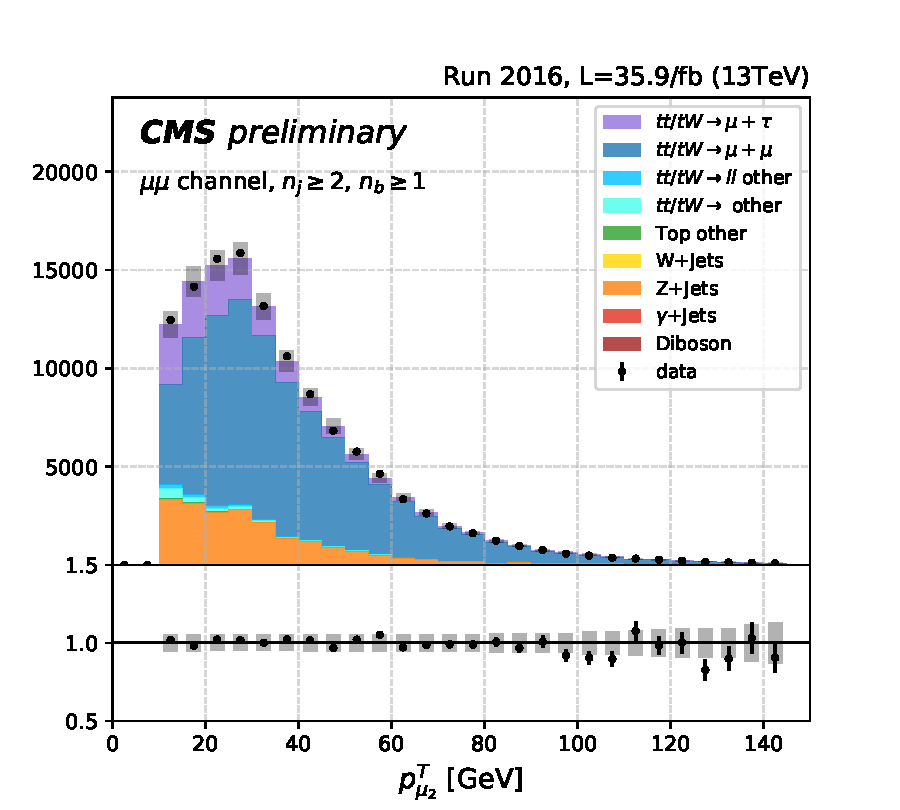
\includegraphics[width=0.9\textwidth]{chapters/Analysis/sectionPlots/figures/kinematics_pickles/mumu/12b/mumu_2b_lepton2_pt.pdf}
            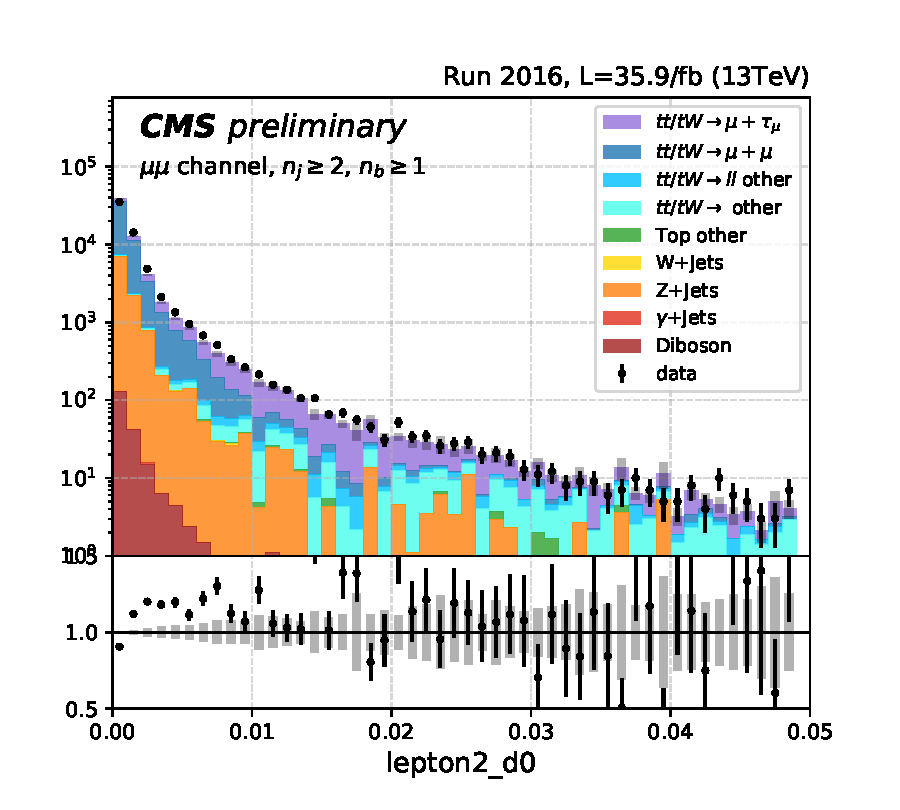
\includegraphics[width=0.9\textwidth]{chapters/Analysis/sectionSelection/figures/sob/mumu_lepton2_d0_logscale.pdf}
        \end{center}

    \end{columns}

\end{frame}


\begin{frame}{\smaller Shape analysis approach -- binned Maximum Likelihood Estimation}

    \begin{tcolorbox}[]{}
        \smaller\smaller 
        In this case, the W branching fractions, $\mathbf{B}$, are
        treated as free parameters, and the values that minimize the NLL
        assuming Poisson probabilities are determined,

        \begin{equation}
            \nonumber
            \mathsf{NLL}(\boldsymbol{B}, \boldsymbol{\theta}|\mathbf{y}) = \sum_{\mathsf{i\in category}} 
            \sum_{\mathsf{j \in bins}} -y_{ij}\ln(f_{ij}(\boldsymbol{B},
            \boldsymbol{\theta})) + f_{ij}(\boldsymbol{B}, \boldsymbol{\theta}) + \sum_{k\in
            n.p.}\pi_\theta (\theta)
        \end{equation}

        where $y_{ij}$ is the data yield in category $i$ and bin $j$, and $f_{ij}$ is the prediction
        parameterized by the branching fractions, $\mathbf{B}$ and nuisance parameters,
        $\boldsymbol{\theta}$. The constraint on the n.p. are denoted by $\pi_{\theta}(\theta)$. The
        data model is written, 

        \begin{equation}
            \nonumber
            f_{ij}(\boldsymbol{B}, \boldsymbol{\theta}) =
            \sum_{s\in sig} s_{ij,s}(\boldsymbol{B}, \boldsymbol{\theta}) + \sum_{b\in bg}
            b_{ij,b}(\boldsymbol{\theta}). 
        \end{equation}

    \end{tcolorbox}

        \begin{itemize}
            \smaller\smaller
            \item 30 categories based on jet and b tag multiplicities 
            \item total of 72 template components, w/ only $\sim 10$ are
                relevant to any specific category
            \item $\sim 100$ non-MC stat nuisance parameters
            \item $\sim 400$ bins in total 
            \item template morphing and MC stat. variation implemented according to arXiv:1103.0354
            \item minimization using \textcolor{blue}{\texttt{scipy.optimize.minimize}}
        \end{itemize}
    
\end{frame}



\begin{frame}{Post-fit distributions} %$ee$ and $\mu\mu$: trailing lepton $\pt$}

    \begin{columns}

        \column{0.5\textwidth}
        \begin{tcolorbox}{\smaller $ee$ and $\mu\mu$: trailing lepton $\pt$}
            \begin{center}
                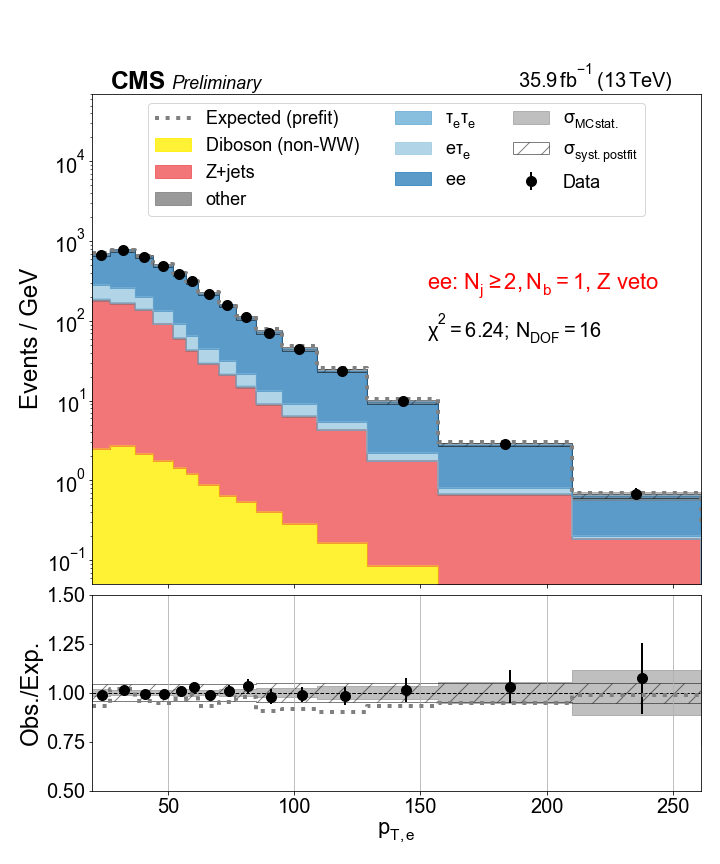
\includegraphics[width=0.48\textwidth]{chapters/Analysis/sectionStatisticalAnalysis/figures/fit/ee_cat_gt2_eq1_b}
                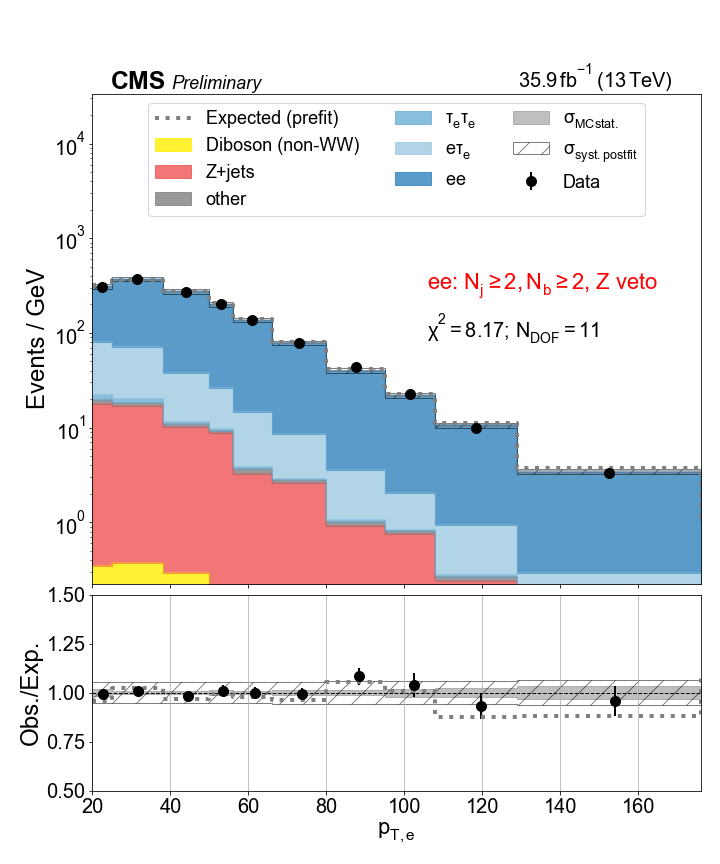
\includegraphics[width=0.48\textwidth]{chapters/Analysis/sectionStatisticalAnalysis/figures/fit/ee_cat_gt2_gt2_b}

                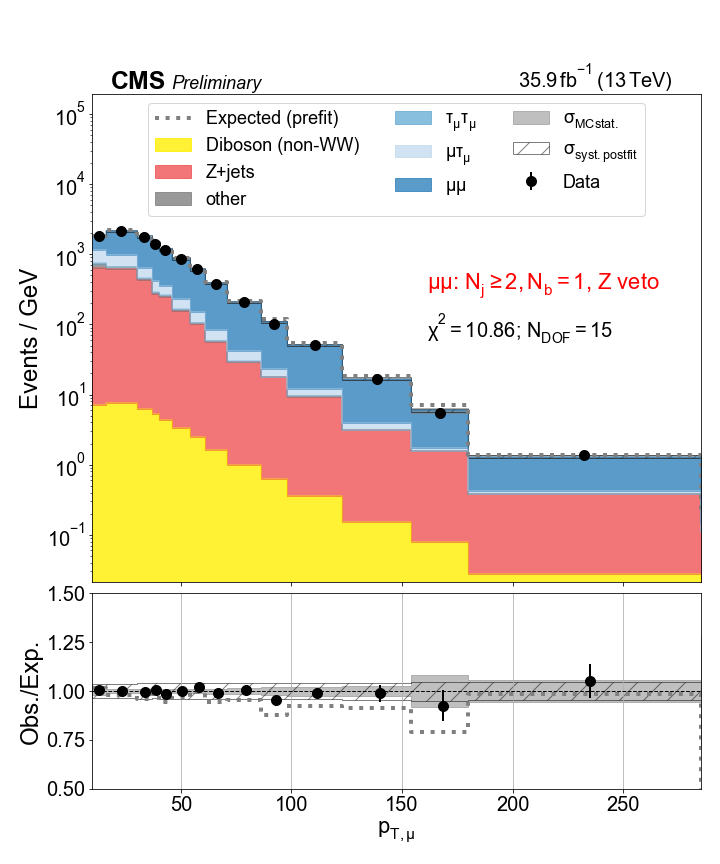
\includegraphics[width=0.48\textwidth]{chapters/Analysis/sectionStatisticalAnalysis/figures/fit/mumu_cat_gt2_eq1_b}
                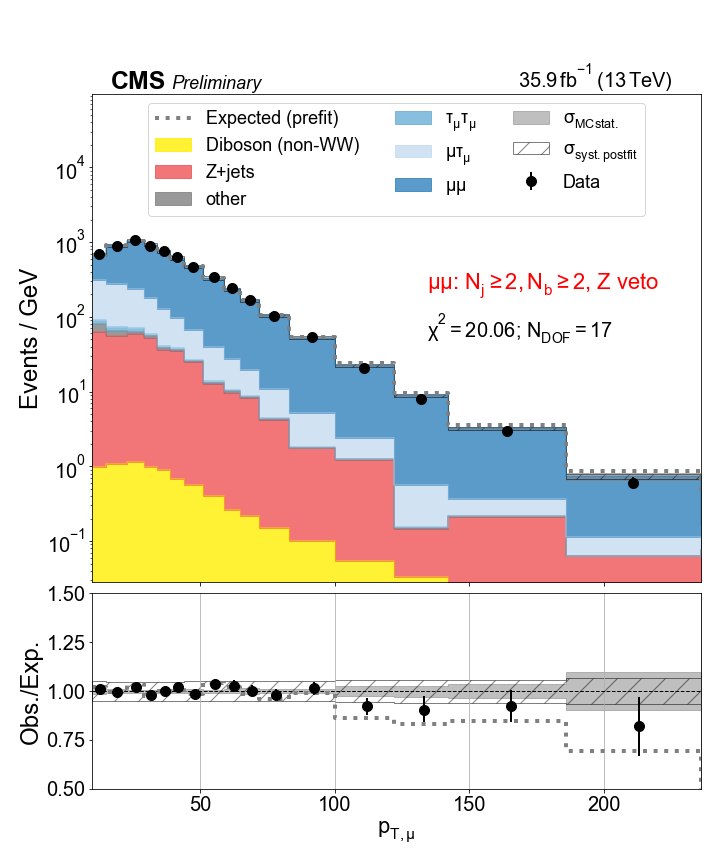
\includegraphics[width=0.48\textwidth]{chapters/Analysis/sectionStatisticalAnalysis/figures/fit/mumu_cat_gt2_gt2_b}
            \end{center}
        \end{tcolorbox}{}

        \column{0.5\textwidth}
        \begin{tcolorbox}{\smaller $e$+jets and $\mu$+jets: lepton $\pt$}
            \begin{center}
                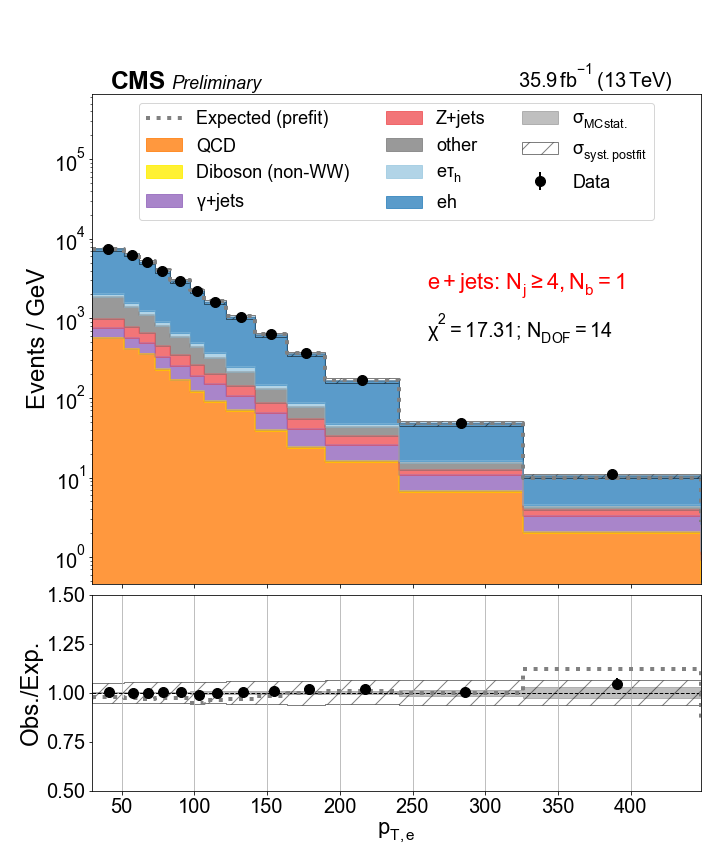
\includegraphics[width=0.48\textwidth]{chapters/Analysis/sectionStatisticalAnalysis/figures/fit/ejet_cat_gt4_eq1}
                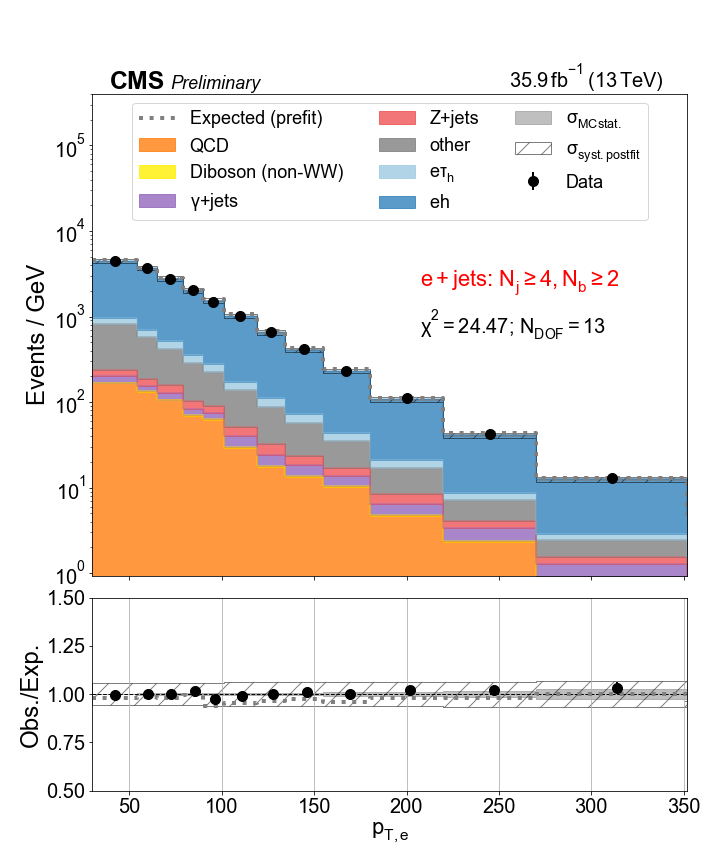
\includegraphics[width=0.48\textwidth]{chapters/Analysis/sectionStatisticalAnalysis/figures/fit/ejet_cat_gt4_gt2}

                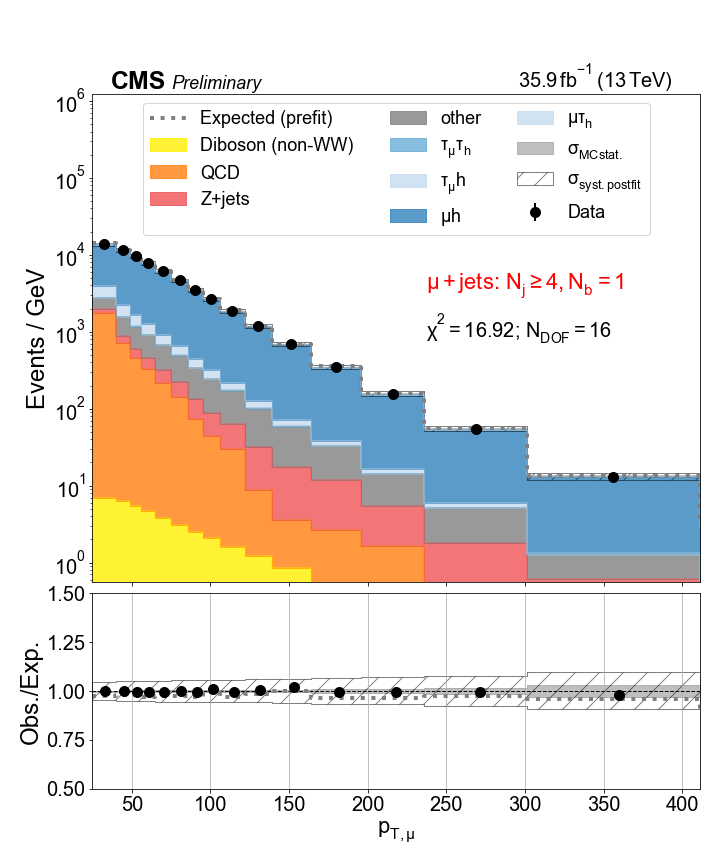
\includegraphics[width=0.48\textwidth]{chapters/Analysis/sectionStatisticalAnalysis/figures/fit/mujet_cat_gt4_eq1}
                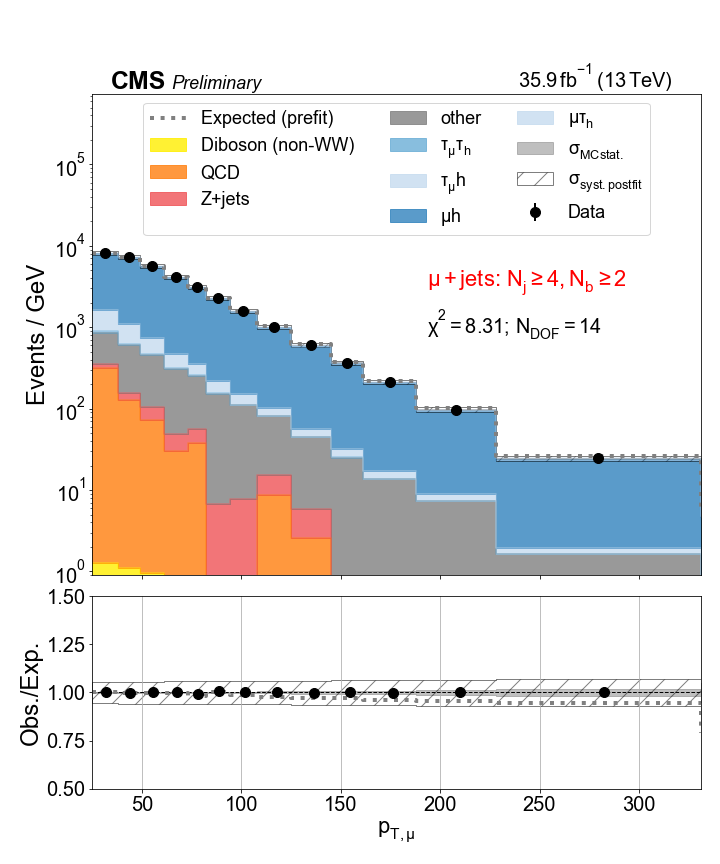
\includegraphics[width=0.48\textwidth]{chapters/Analysis/sectionStatisticalAnalysis/figures/fit/mujet_cat_gt4_gt2}
            \end{center}
        \end{tcolorbox}
    \end{columns}

\end{frame}

\begin{frame}{Post-fit distributions}

    \begin{tcolorbox}{$e\mu$: trailing lepton $\pt$}
        \begin{center}
            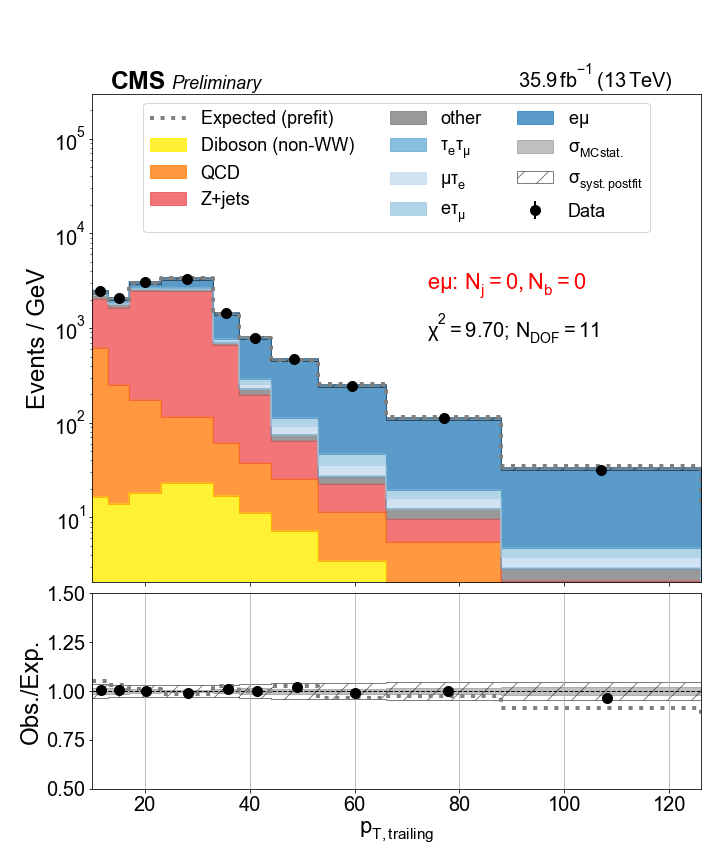
\includegraphics[width=0.25\textwidth]{chapters/Analysis/sectionStatisticalAnalysis/figures/fit/emu_cat_eq0_eq0_a}
            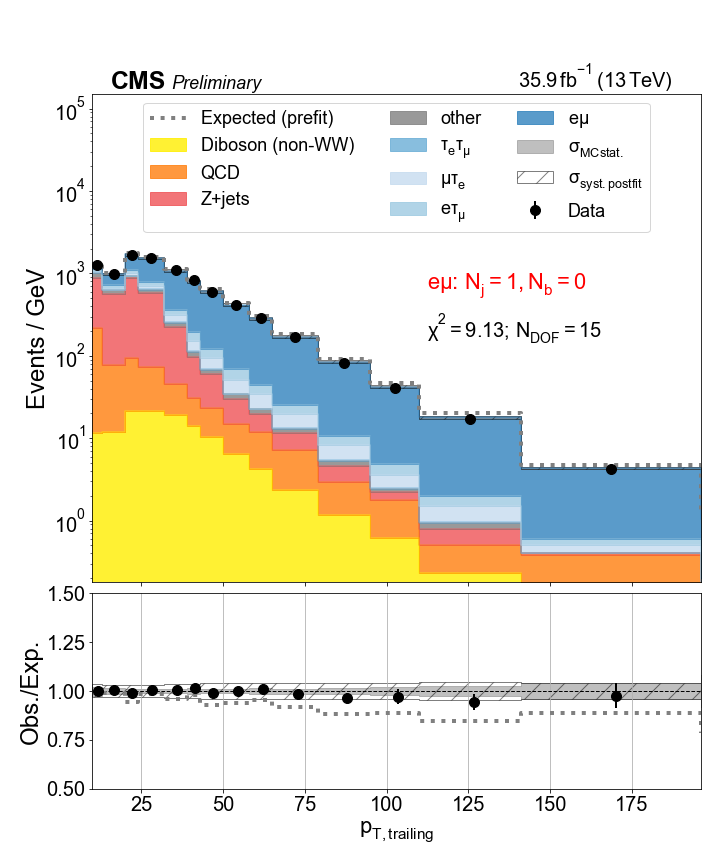
\includegraphics[width=0.25\textwidth]{chapters/Analysis/sectionStatisticalAnalysis/figures/fit/emu_cat_eq1_eq0_a}
            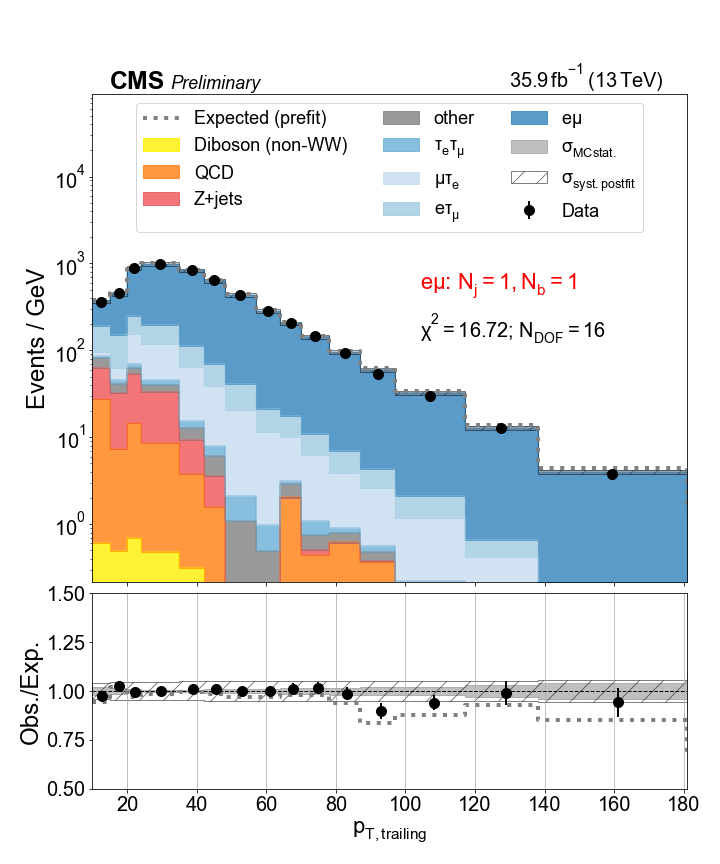
\includegraphics[width=0.25\textwidth]{chapters/Analysis/sectionStatisticalAnalysis/figures/fit/emu_cat_eq1_eq1_a}

            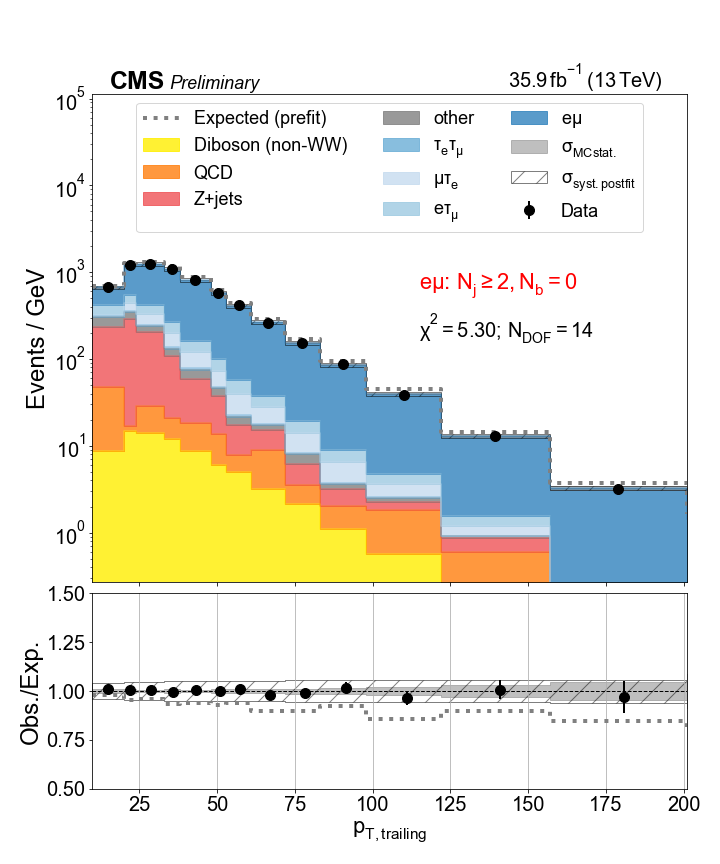
\includegraphics[width=0.25\textwidth]{chapters/Analysis/sectionStatisticalAnalysis/figures/fit/emu_cat_gt2_eq0}
            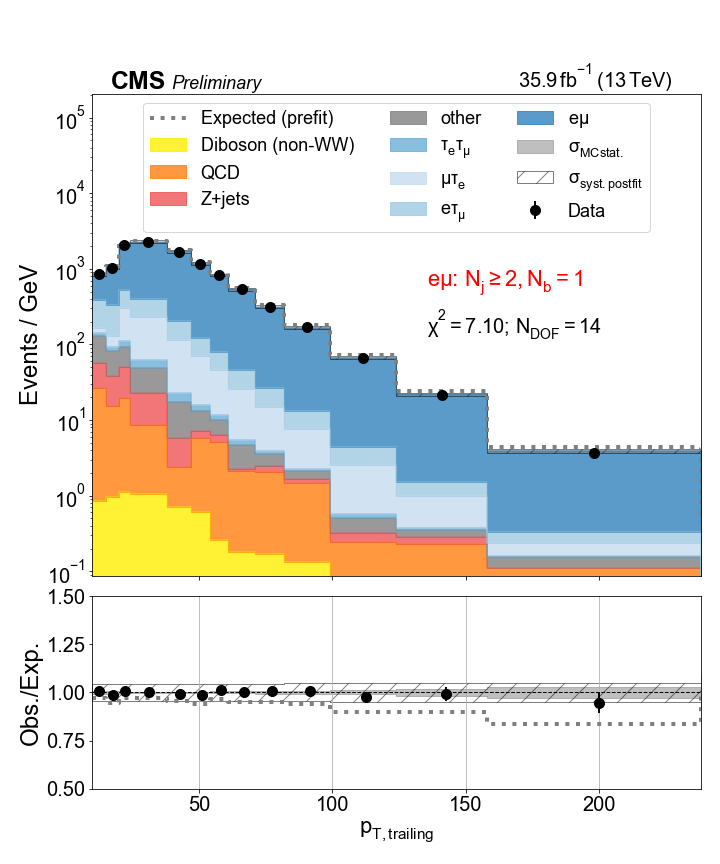
\includegraphics[width=0.25\textwidth]{chapters/Analysis/sectionStatisticalAnalysis/figures/fit/emu_cat_gt2_eq1_a}
            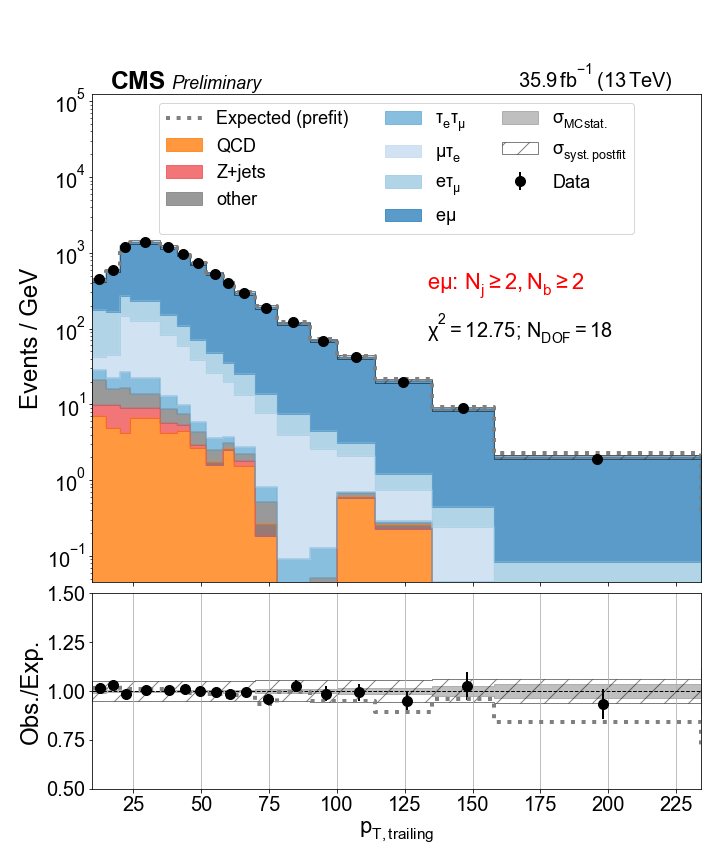
\includegraphics[width=0.25\textwidth]{chapters/Analysis/sectionStatisticalAnalysis/figures/fit/emu_cat_gt2_gt2_a}
        \end{center}
    \end{tcolorbox}

\end{frame}

\begin{frame}{Post-fit distributions}

    \begin{tcolorbox}{$e\tau$: $\tau_{h}\,\pt$}
        \begin{center}
            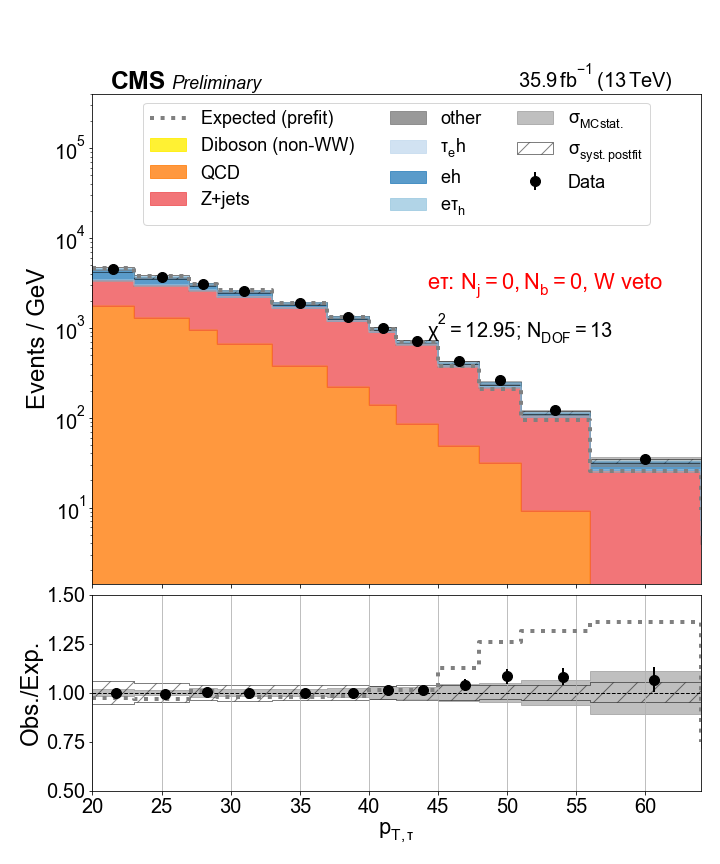
\includegraphics[width=0.24\textwidth]{chapters/Analysis/sectionStatisticalAnalysis/figures/fit/etau_cat_eq0_eq0}
            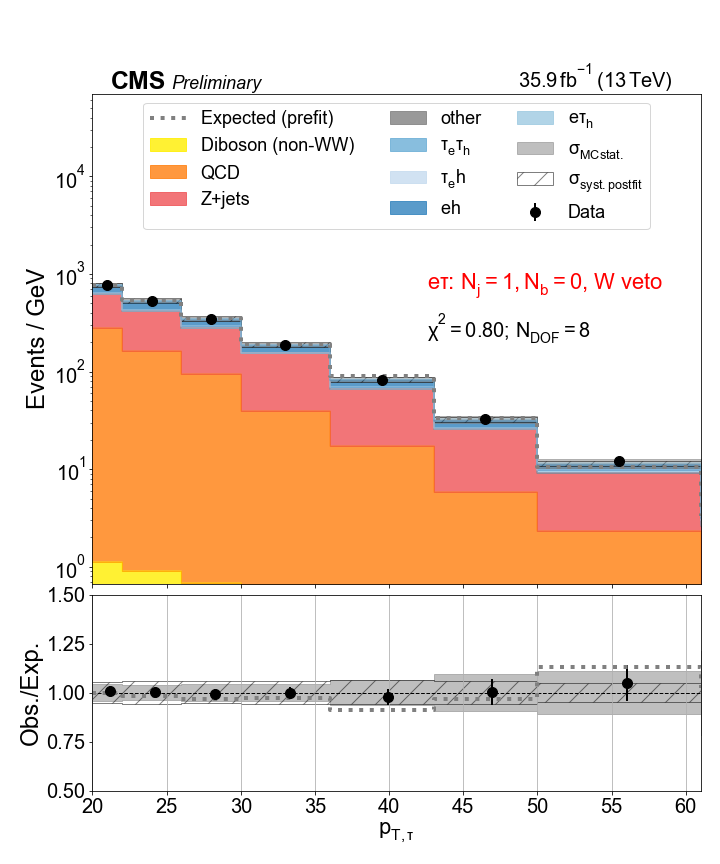
\includegraphics[width=0.24\textwidth]{chapters/Analysis/sectionStatisticalAnalysis/figures/fit/etau_cat_eq1_eq0}
            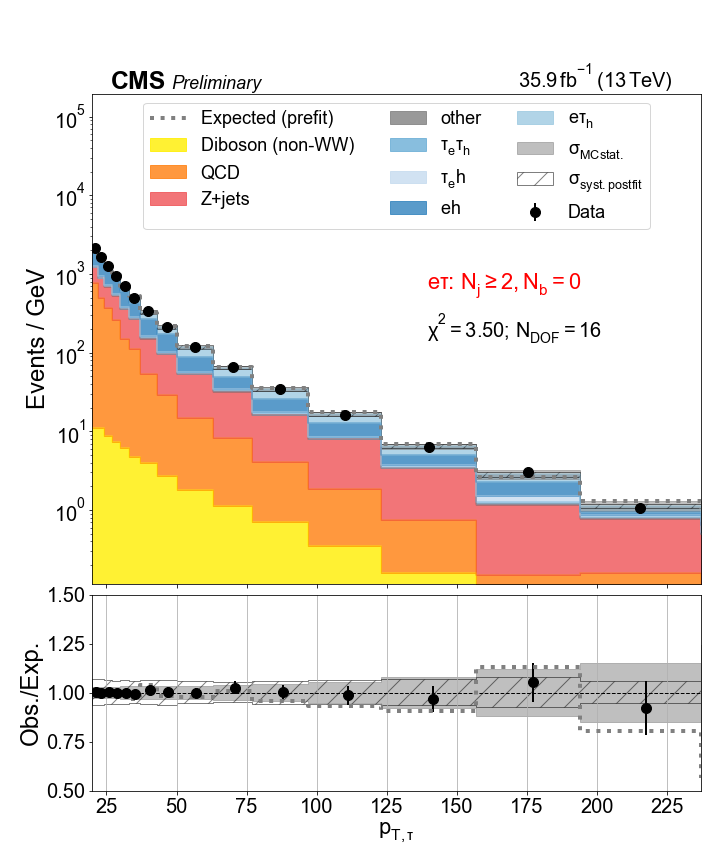
\includegraphics[width=0.24\textwidth]{chapters/Analysis/sectionStatisticalAnalysis/figures/fit/etau_cat_gt2_eq0}
            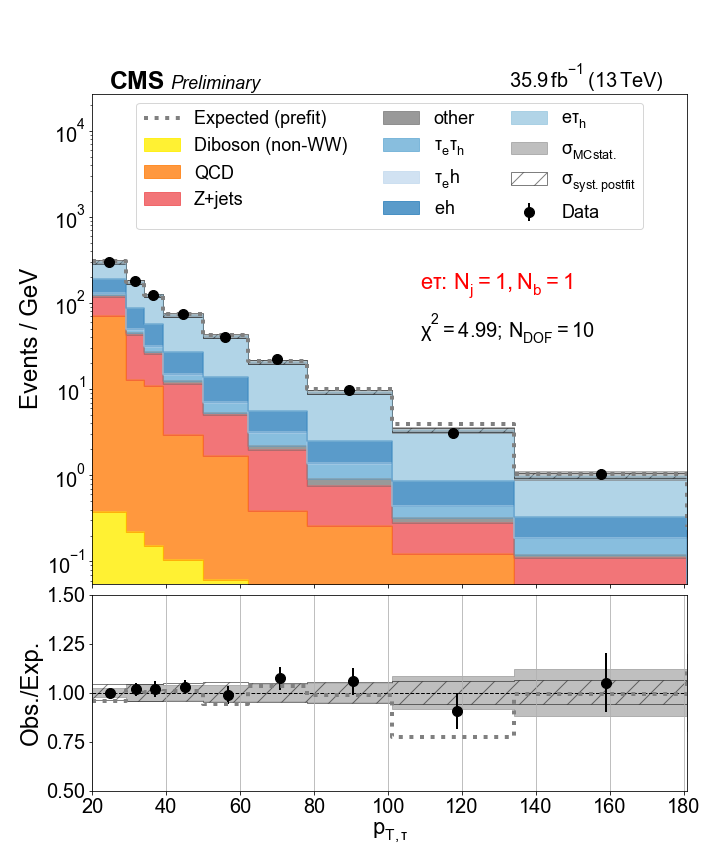
\includegraphics[width=0.24\textwidth]{chapters/Analysis/sectionStatisticalAnalysis/figures/fit/etau_cat_eq1_eq1}

            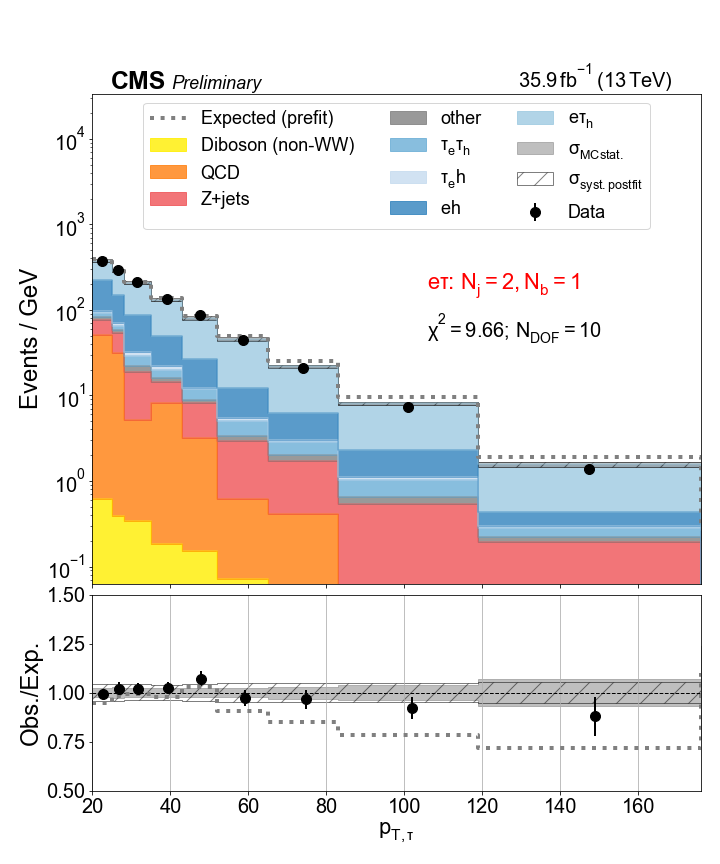
\includegraphics[width=0.24\textwidth]{chapters/Analysis/sectionStatisticalAnalysis/figures/fit/etau_cat_eq2_eq1}
            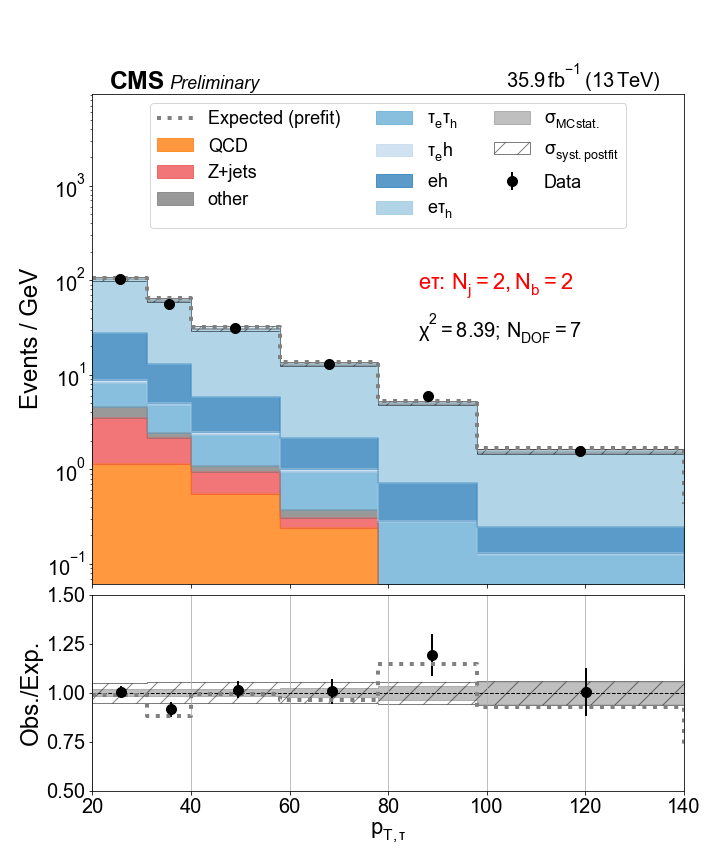
\includegraphics[width=0.24\textwidth]{chapters/Analysis/sectionStatisticalAnalysis/figures/fit/etau_cat_eq2_eq2}
            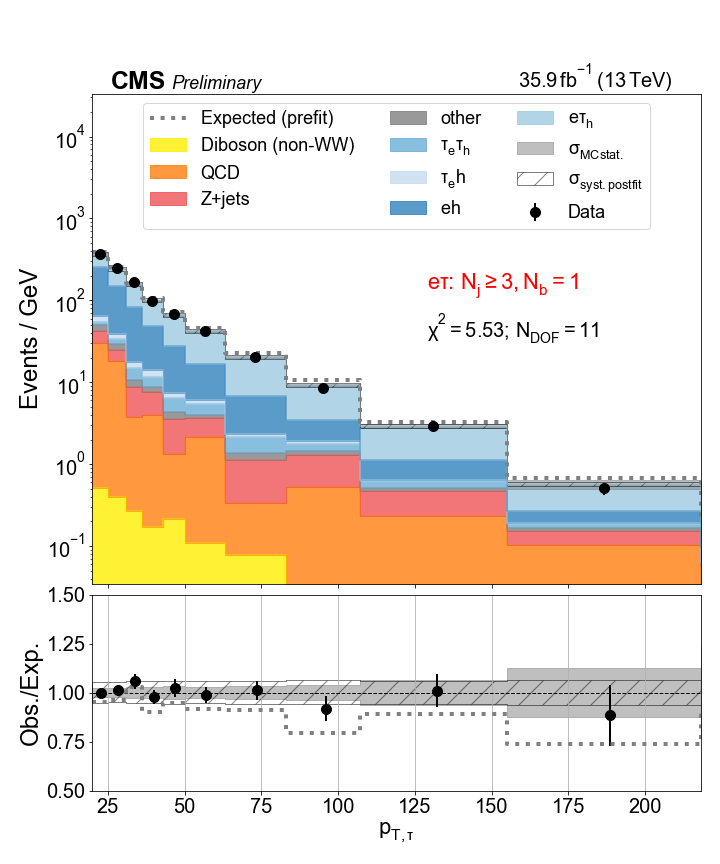
\includegraphics[width=0.24\textwidth]{chapters/Analysis/sectionStatisticalAnalysis/figures/fit/etau_cat_gt3_eq1}
            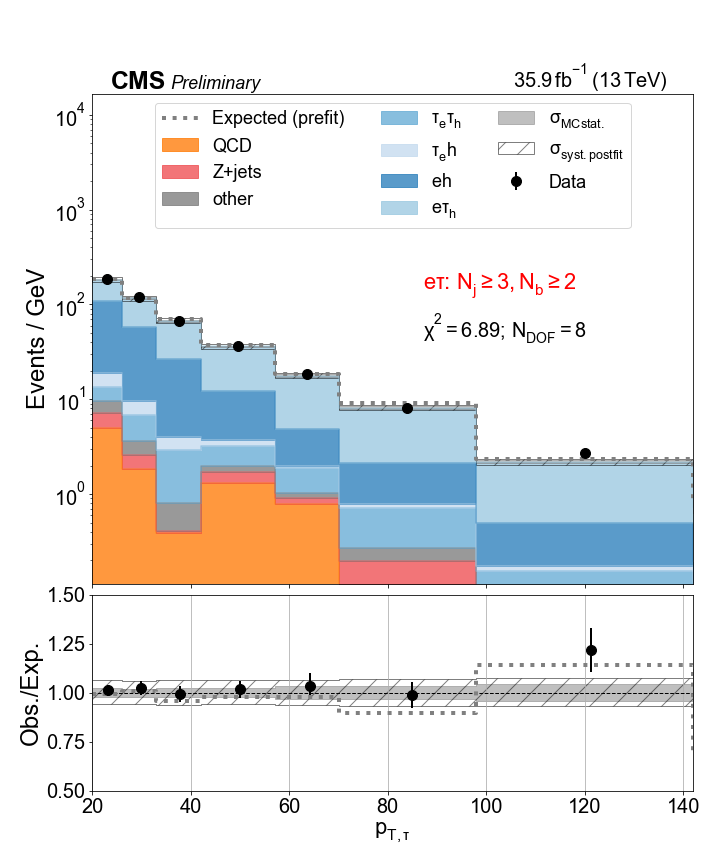
\includegraphics[width=0.24\textwidth]{chapters/Analysis/sectionStatisticalAnalysis/figures/fit/etau_cat_gt3_gt2}
        \end{center}
    \end{tcolorbox}
\end{frame}

\begin{frame}{Post-fit distributions}

    \begin{tcolorbox}{$\mu\tau$: $\tau_{h}\,\pt$}
        \begin{center}
            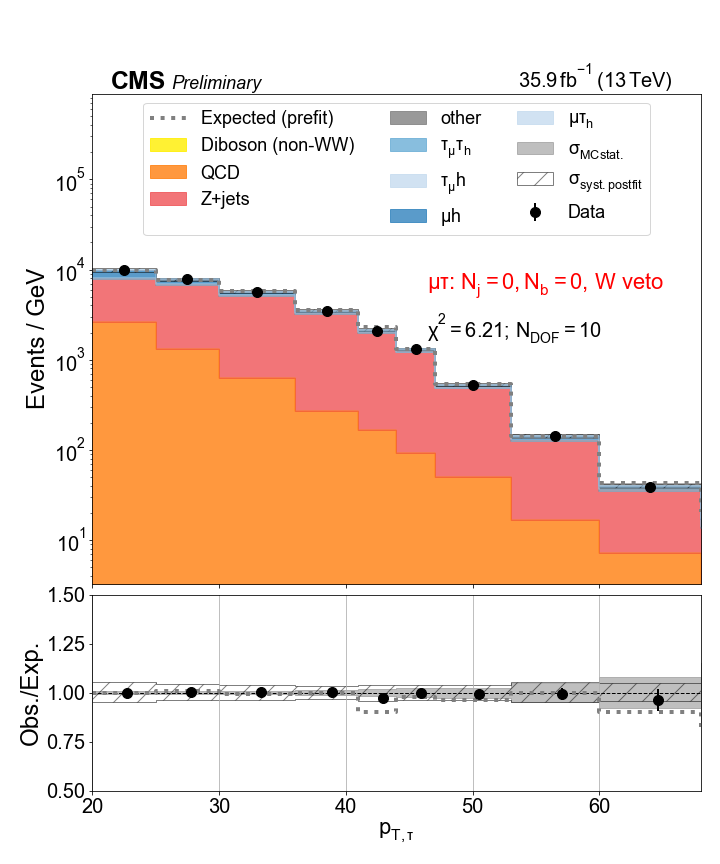
\includegraphics[width=0.24\textwidth]{chapters/Analysis/sectionStatisticalAnalysis/figures/fit/mutau_cat_eq0_eq0}
            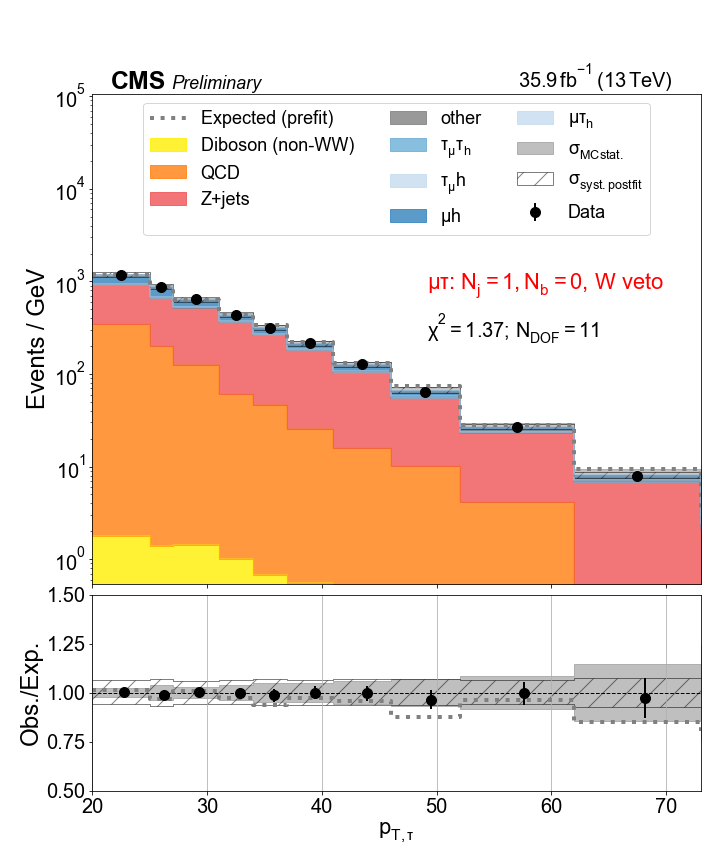
\includegraphics[width=0.24\textwidth]{chapters/Analysis/sectionStatisticalAnalysis/figures/fit/mutau_cat_eq1_eq0}
            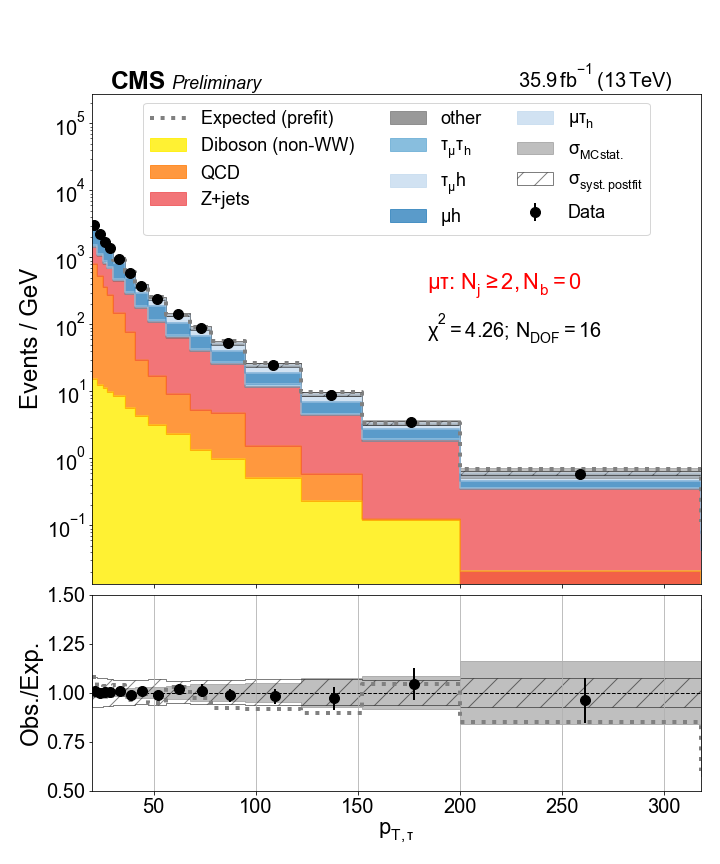
\includegraphics[width=0.24\textwidth]{chapters/Analysis/sectionStatisticalAnalysis/figures/fit/mutau_cat_gt2_eq0}
            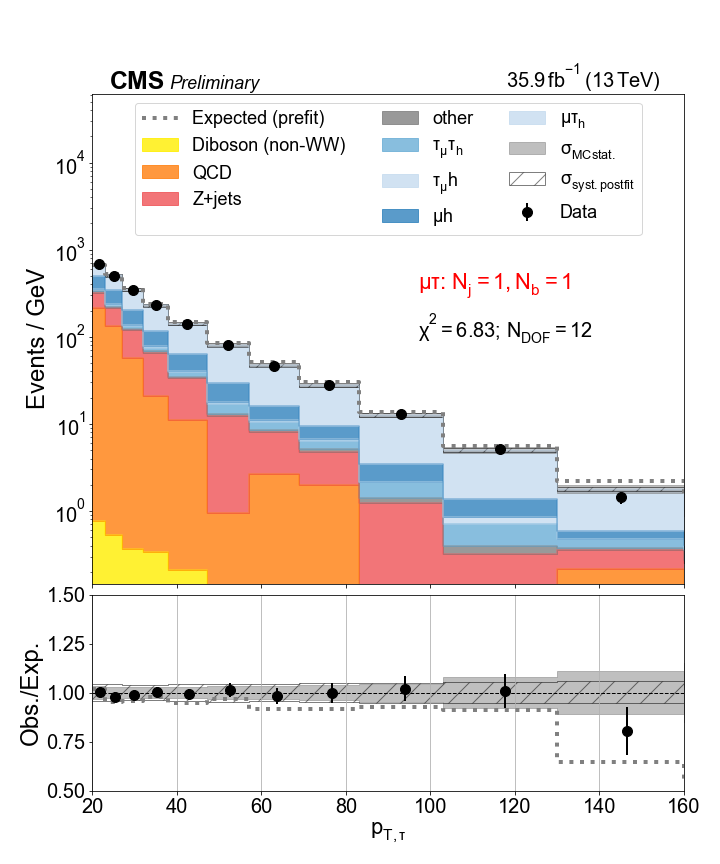
\includegraphics[width=0.24\textwidth]{chapters/Analysis/sectionStatisticalAnalysis/figures/fit/mutau_cat_eq1_eq1}

            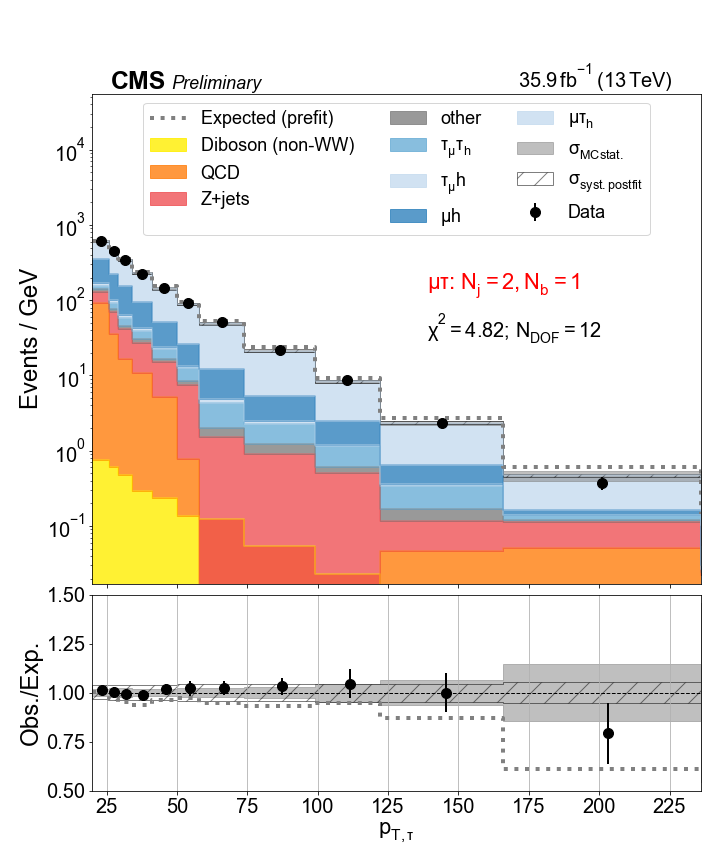
\includegraphics[width=0.24\textwidth]{chapters/Analysis/sectionStatisticalAnalysis/figures/fit/mutau_cat_eq2_eq1}
            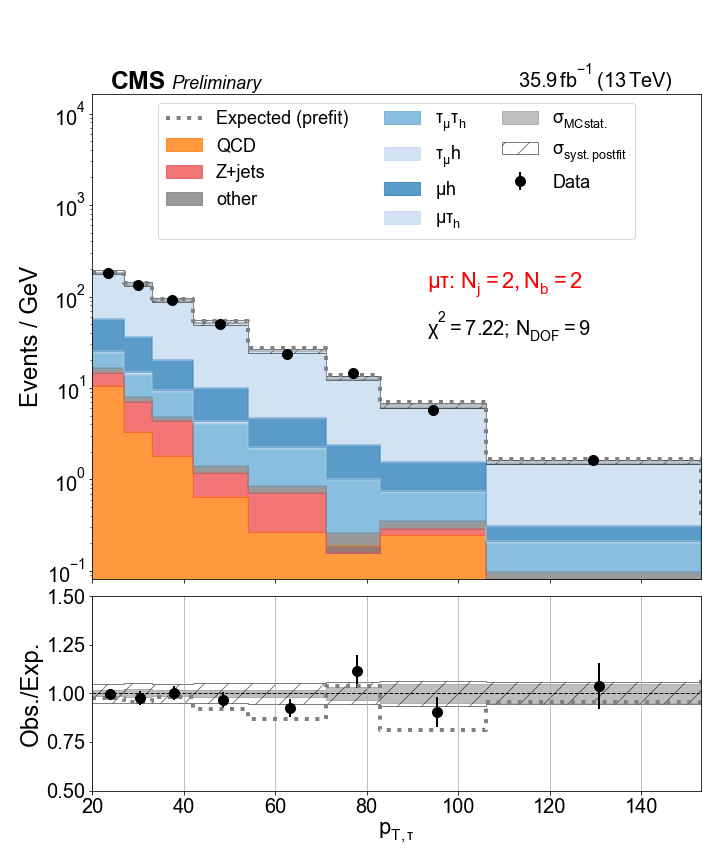
\includegraphics[width=0.24\textwidth]{chapters/Analysis/sectionStatisticalAnalysis/figures/fit/mutau_cat_eq2_eq2}
            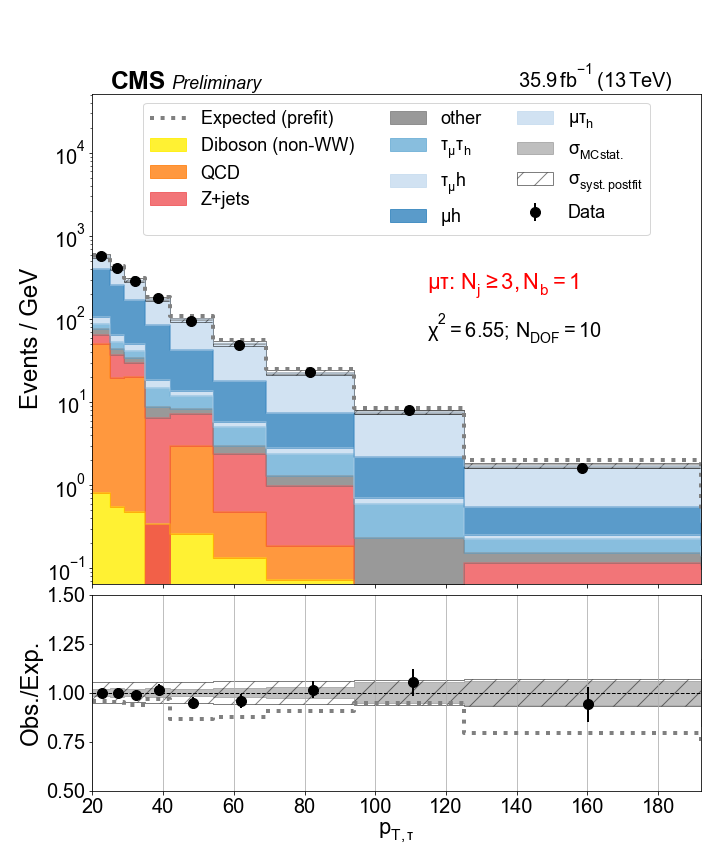
\includegraphics[width=0.24\textwidth]{chapters/Analysis/sectionStatisticalAnalysis/figures/fit/mutau_cat_gt3_eq1}
            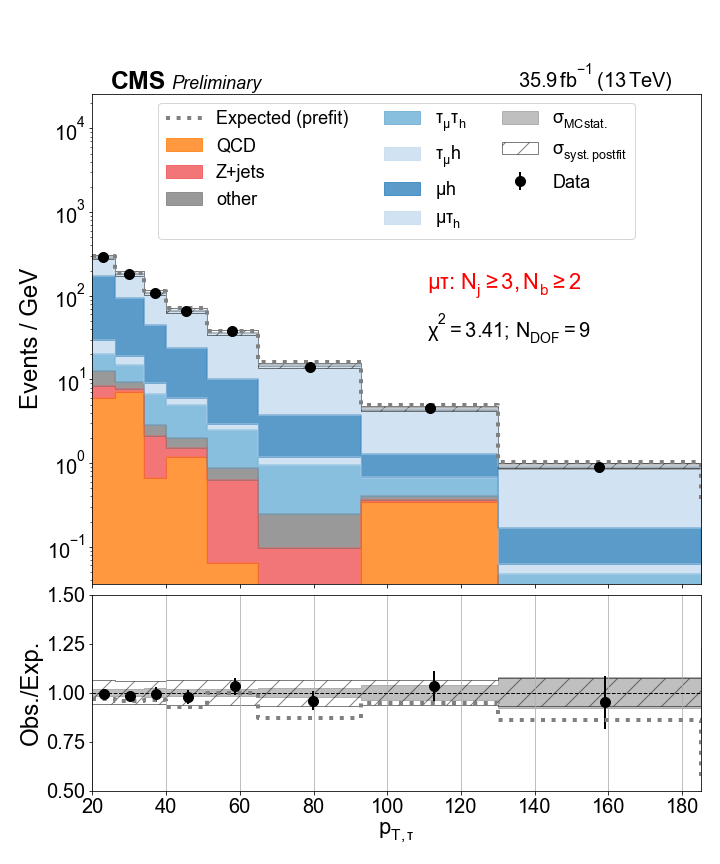
\includegraphics[width=0.24\textwidth]{chapters/Analysis/sectionStatisticalAnalysis/figures/fit/mutau_cat_gt3_gt2}
        \end{center}
    \end{tcolorbox}

\end{frame}
